% ------------------------------------------------------------------------
% ------------------------------------------------------------------------
% abnTeX2: Modelo de Trabalho Acadêmico (tese de doutorado, dissertação de
% mestrado e trabalhos monográficos em geral) em conformidade com 
% as normas da ABNT
% ------------------------------------------------------------------------
% ------------------------------------------------------------------------

\documentclass[english, 
               brazil, 
               msc] %Opções bsc (TCC) e msc (Mestrado)
               {dcomp-abntex2}

% Geração de dummy text
% Retirar para a versão final do documento
\usepackage{lipsum}


%Compila o indice
\makeindex

\begin{document}

% Seleciona o idioma do documento (conforme pacotes do babel)
\selectlanguage{brazil}

% Retira espaço extra obsoleto entre as frases.
\frenchspacing 

% ----------------------------------------------------------
% ELEMENTOS PRÉ-TEXTUAIS
% ----------------------------------------------------------
\pretextual

\titulo{Utilizando Algoritmos Mágicos para Resolver Problemas de Bancos de dados Obscuros em Nuvens Cumulonimbus}
\autor{Arnold Schwarzenegger da Silva}
\orientador{Andrew S. Tanenbaum}
\coorientador{Donald Knuth}
\curso{Ciência da Computação}

\imprimircapa
\imprimirfolhaderosto*

\imprimirfichacatalografica
\imprimirfolhadeaprovacao
    
\begin{dedicatoria}
   \vspace*{\fill}
   \centering
   \noindent
   \textit{ Dedico este trabalho primeiramente a Deus, que é meu guia; à toda minha família, principalmente, minha mãe, que me deu todo apoio, compreendendo minhas ausências ao longo dos períodos; ao meu namorado, Gabriel, que também esteve sempre ao meu lado me motivando durante minhas dificuldades e me compreendendo; aos meus amigos de curso, que também estiveram presentes nos desafios do curso, fracassos e sucessos; e aos professores que me deram orientação e todo o suporte para que eu chegasse aqui.} \vspace*{\fill}
\end{dedicatoria}
% ---
\begin{agradecimentos}

%lipsum[1-4] 
 Agradeço ao Prof. Ricardo José Paiva de Britto Salgueiro e à Prof. Edilayne Meneses Salgueiro por me orientarem na produção deste trabalho e por me motivarem a continuar trilhando o caminho da educação e da pesquisa. Agradeço também à Marco Aurélio Cruz Fonseca, que percorreu comigo os desafios deste trabalho, me ensinando e também aprendendo junto a mim.
\end{agradecimentos}
% ---
\begin{epigrafe}[]
    \vspace*{\fill}
	\begin{flushright}
	
		\textit{
				“A verdadeira viagem de descobrimento \\ não consiste em procurar novas paisagens,\\ mas em ter novos olhos”. (Marcel Proust)
				}
		
	\end{flushright}
\end{epigrafe}
% ---
% resumo em português
\setlength{\absparsep}{18pt} % ajusta o espaçamento dos parágrafos do resumo
\begin{resumo}
  


 \textbf{Palavras-chave}: 
\end{resumo}
% resumo em inglês
\setlength{\absparsep}{18pt} % ajusta o espaçamento dos parágrafos do resumo
\begin{resumo}[Abstract]
 \begin{otherlanguage*}{english}
   

   \textbf{Keywords}: Algorithms, DataBase, Cloud Computing, Lero-Lero.
 \end{otherlanguage*}
\end{resumo}
    
% Lista de Figuras
\pdfbookmark[0]{\listfigurename}{lof}
\listoffigures*
\cleardoublepage

% Lista de Tabelas
\pdfbookmark[0]{\listtablename}{lot}
\listoftables*
\cleardoublepage

% Lista de Códigos
\pdfbookmark[0]{\listlistingname}{lol}
\begin{KeepFromToc}
	\listoflistings
\end{KeepFromToc}
\cleardoublepage
   
% ---
% inserir lista de abreviaturas e siglas
% ---

\begin{siglas}
    \item[SDN]{Software-Defined Networking}
	\item[API]{Application Programming Interface}
	\item[DoS]{Denial of Servie}
	\item[IP]{Internet Protocol}
	\item[MAC]{Media Acess Control}
	\item[RFC]{Requests for Comments}
	\item[PC]{Personal Computer}
	\item[WAN]{Wide Area Network}
	\item[NIB]{Network Information Base}
	\item[AMQP]{Advanced Message Queuing Protocol}
	\item[RSVP]{Resource Reservation Protocol}
	\item[REST]{Representational State Transfer}
	\item[WEB]{World Wide Web}
	\item[VM]{Virtual Machine}

\end{siglas}
% ---
% ---
% inserir lista de símbolos
% ---

\begin{simbolos}
  \item[$ \Gamma $] Letra grega Gama
  \item[$ \Lambda $] Lambda
  \item[$ \zeta $] Letra grega minúscula zeta
  \item[$ \in $] Pertence
\end{simbolos}
% ---
    
\pdfbookmark[0]{\contentsname}{toc}
\tableofcontents*
\cleardoublepage

% ----------------------------------------------------------
% ELEMENTOS TEXTUAIS
% ----------------------------------------------------------
\textual
\chapter{Introdução}

\section{Contextualização}

O desenvolvimento das redes tradicionais de computadores, principalmente, quando se fala em redes corporativas, envolve o aumento da infraestrutura física, o que implica também no aumento da complexidade de gerenciamento de elementos físicos como roteadores e \emph{switches}. Os equipamentos mais modernos normalmente são formados pela camada ou plano de controle e de dados, os quais possuem funções diferentes. A camada de controle é responsável pela lógica de encaminhamento dos dados no nível físico, logo, ele dita como o \emph{switch} deve lidar com os dados que passarem por ele. O plano de dados já é responsável por lidar com os dados propriamente ditos, os encaminhando para outros \emph{switches} e cumprindo com o que lhe foi atribuído pelo plano de controle. O maior desafio para as redes convencionais se encontra no fato que os elementos físicos possuem seus planos de controle configurados pelo próprio fabricante. Nesse contexto, quando se fala em redes heterogêneas, o gerenciamento se torna muito mais complexo para os administradores, que precisam lidar com diferentes tecnologias e diferentes protocolos. Esse desafio limita o desenvolvimento de experimentos e novas tecnologias para redes, tornando necessário que se estude novas abordagens que solucionem essa limitação.
\par As Redes Definidas por Software surgiram neste cenário como solução para esses problemas decorrentes nas redes convencionais. As ideias por trás das redes programáveis surgiram a partir do final dos anos 90 com as redes ativas. Já por volta do início dos anos 2000 surgiu o conceito da separação dos plano de controle e de dados, uma das principais características das redes SDN. A partir de 2007, o projeto Ethane deu início à utilização de interfaces abertas nas redes SDN, possibilitando que o OpenFlow fosse implementado e posteriormente fosse viabilizado como interface \emph{SouthBound} padrão das redes SDN.\cite{Feamster:2013:RS:2559899.2560327} Dessa forma, as Redes Definidas por Software chegaram à arquitetura atual, onde o plano de controle é responsabilidade dos controladores SDN e o plano de dados permaneceu em função dos elementos físicos de encaminhamento, como roteadores e \emph{switches}.
\par Por ser tão recente, as redes SDN ainda enfrentam muitos desafios, principalmente em torno da segurança de dados. Isso se deve porque as soluções atualmente existentes levam em consideração ataques nas redes tradicionais e a segurança não é uma característica inerente à arquitetura SDN. Além da modificação das ameaças das redes tradicionais, novas ameaças surgiram devido às próprias características do SDN, como centralização lógica e programabilidade da rede. Atualmente, já existem soluções que se concentram em fornecer segurança a partir de novas políticas administrativas, aplicações ligadas aos controladores e até modificações na própria arquitetura SDN.
\par Além dos desafios em torno da segurança, um outro ponto constantemente debatido é em relação à disposição dos controladores em uma rede.Sabe-se que utilizar somente um controlador, pode gerar problemas relacionados à sobrecarga do mesmo, principalmente em redes complexas. A partir de então, sugeriu-se a utilização de mais controladores, que compartilham a visão global da rede podendo se dispor de forma hierárquica ou não. Entretanto, a forma como isso deve ocorrer e como esses controladores devem se comunicar ainda é motivo de estudos e experimentos.
\par Neste contexto, este trabalho tem como propósito desenvolver um gerenciador para 2 controladores SDN em uma rede distribuída, utilizando os serviços de segurança implementados por \citeonline{pablo} e \citeonline{bomfim2}.  

\section{Objetivos}

\subsection{Objetivo Geral}

Desenvolver um gerenciador SDN para dois controladores com diferentes implementações e utilizando serviços com propósitos de segurança.

\subsection{Objetivos Específicos}

\begin{itemize}
    \item Analisar arquitetura dos controladores a serem gerenciados;
    \item Projetar módulo de gerenciamento para 2 controladores pré-definidos, elicitando seus requisitos, de forma que seja escalável para outros controladores;
    \item Analisar performance desse controlador;
\end{itemize}


\section{Estrutura do Documento}

Para facilitar a navegação e melhor entendimento, este documento está estruturado com os seguintes capítulos:
\begin{itemize}
\item {Capítulo 1 - Introdução} 
\item {Capítulo 2 - Fundamentação Teórica}
\item {Capítulo 3 - Trabalhos Relacionados}
\item {Capítulo 4 - Metodologia}
\end{itemize}

\chapter{Trabalhos Relacionados}

É inerente ao paradigma SDN a centralização lógica da rede em um único controlador. Entretanto, devido à variedade de serviços prestados e ao possível crescimento da infraestrutura de redes, projetar um plano de controle distribuído tornou-se uma opção a ser analisada para evitar o gargalo em um único controlador. O OpenFlow, apesar de ser o padrão de interface para comunicação entre plano de dados e controle, não possui uma definição para comunicação entre controladores para o caso de um plano de controle distribuído. Esta seção apresenta alguns trabalhos com possíveis soluções para o gerenciamento de controladores distribuídos..

\section{HyperFlow}

O trabalho de \citeonline{hiperflow} foi o primeiro a propor uma aplicação para o plano de controle distribuído: o HiperFlow. Essa solução foi implementada como uma aplicação específica no controlador NOX, dessa forma, para utilizá-lo de forma distribuída deve-se instanciar todos os controladores dentro da mesma rede OpenFlow de forma que  cada instância controle um certo número de \emph{switches} e cada \emph{switch} seja controlado por somente um controlador, como ilustra a Figura \ref{hyperflow}.
\par O funcionamento do Hyperflow é baseado em eventos, assim, a aplicação em uma instância é responsável por capturar todos os eventos ocorridos em sua área e em seguida divulgá-los aos outros controladores utilizando o paradigma publicação/assinatura. Para realizar essa divulgação o HyperFlow utiliza o WheelFS\cite{Stribling}, um sistema de arquivos projetado especificamente para armazenamento de arquivos em sistemas distribuídos. Dessa forma, o HyperFlow somente define um diretório como canal de comunicação dos eventos,checando-o periodicamente por possíveis mudanças, e estes serão divulgados pelo WheelFs através de arquivos neste mesmo diretório. 

\pagebreak
\begin{figure}[!h]
	\caption{ Arquitetura do HyperFlow}
  \centering
  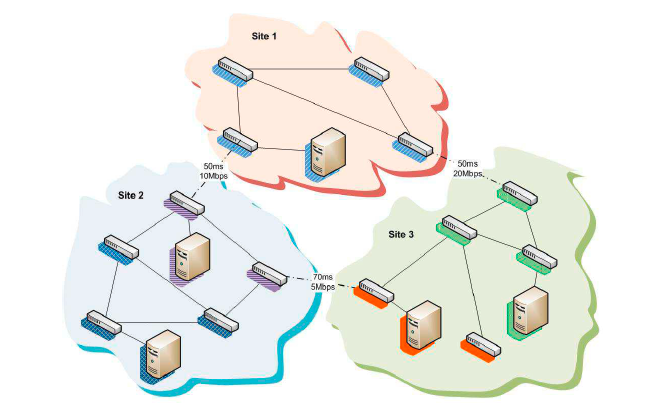
\includegraphics[scale=1]{Imagens/hiperflow.PNG} 
 
  \legend{Fonte: \citeonline{hiperflow}}
  \label{hyperflow}
\end{figure}

\par A partir dessa arquitetura todas as solicitações podem ser atendidas localmente pelos controladores, reduzindo o tráfego entre as áreas e ainda mantendo a visão global da rede. Além disso, caso algum controlador responsável por uma área falhe, outro controlador pode e irá assumir sua função, já que todos as informações necessárias estarão nos arquivos divulgados. O problema citado dessa arquitetura é justamente a necessidade de se implementar diversas instâncias do HyperFlow em cada controlador NOX, implicando em alterar o código no núcleo do controlador para interceptar comandos e serializar eventos.

\section{Onix}

A proposta de \citeonline{onix} consiste no Onix, uma aplicação para controladores distribuídos que se difere de outros trabalhos por expor uma interface mais genérica, tendo como alvo ambientes diversos como redes WAN, nuvens públicas e centros de dados corporativos.Além disso, provê meios para distribuições flexíveis permitindo que os \emph{designers} de aplicações implementem aplicações de controle sem reinventar mecanismos de distribuições e mantendo requisitos de escalabilidade e performance. De acordo com a Figura \ref{onix}, existem 4 componentes em uma rede controlada pelo Onix:

\begin{itemize}
    \item Infraestrutura física: Inclui \emph{switches} e roteadores e outras entidades físicas que permitam que Onix leia e escreva o estado que controla o comportamento do elemento, como em uma espécie de tabela de encaminhamento.
    \item Infraestrutura de conexão: Corresponde à comunicação entre o Onix e a infraestrutura física. Esse canal de controle pode ser implementando tanto na banda(tráfego de controle compartilha a mesma conexão com o tráfego de dados), como fora da banda(tráfego de controle e dados utilizam conexões separadas) e deve fornecer ainda comunicação bidirecional.
    \item Onix: Sistema distribuído que é executado em um cluster composto de um ou mais sevidores físicos, onde cada um pode executar múltiplas instâncias do Onix. O Onix é responsável por fornecer acesso lógico de controle à rede(em ações como escrever e ler o estado da rede) e disseminar o estado da rede para outras instâncias dentro do cluster.
    \item Lógica de controle: A lógica de controle da rede é implementada no topo da interface do Onix. Essa lógica determina o comportamento desejado da rede. O Onix somente fornece os meios necessários para acessar o estado apropriado da rede.
\end{itemize}


\begin{figure}[!h]
	\caption{ Arquitetura do Onix}
  \centering
  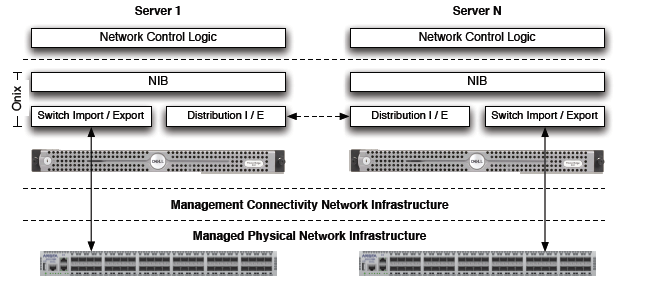
\includegraphics[scale=1]{Imagens/onix.png} 
 
  \legend{Fonte: \citeonline{onix}}
  \label{onix}
\end{figure}

O Onix utiliza um modelo de dados chamado \emph{Network Information Base} (NIB). Este modelo faz o controle do estado da rede através de uma estrutura de dados que armazena um grafo das entidades da topologia da rede. É através da replicação e distribuição desse modelo NIB que o Onix consegue prover a escalabilidade. Para que ocorra a sincronização de dados sem falha entre os processos distribuídos, o Onix utiliza a API Apache Zookeeper, possibilitando que o mesmo mantenha, por exemplo, informações de configuração, nomeação de servidores e provendo serviços para grupos específicos da rede. Apesar de sua contribuição relevante, tendo se baseado no contolador NOX e no Apache ZooKeeper, o Onix foi desenvolvido em código fechado, impossibilitando a integração e o desenvolvimento de novas aplicações.
\pagebreak
\section{DISCO - \emph{DIstributed SDN COntrol Plane} }

O trabalho de \citeonline{disco} apresenta outra possibilidade para integração de controladores DISCO. A implementação se baseia nos controladores Floodlight, cada qual com seu domínio da rede. Por sua vez estes se comunicam para manter uma visão global da rede utilizando uma interface \emph{East/West} através do \emph{Advanced Message Queuing Protocol} (AMQP)\cite{amqp}. O OpenFlow se mantém como interface \emph{SouthBound} para comunicação com a camada de dados da rede.
    O conceito utilizado pelo DISCO é que cada controlador Floodlight possui um agente configurado que permite trocar informações sobre os domínios adjacentes utilizando o AMQP. Essa API é composta de um módulo que identifica os controladores vizinhos, possibilitando a troca de mensagens. Entre os agentes descritos temos:
    
    \begin{itemize}
        \item O agente de conectividade, responsável pelo peering;
        \item O agente de monitoramento, responsável por buscar informações sobre largura de banda e latência;
        \item O agente de acessibilidade, responsável por avisar caso apareça um novo host no domínio;
        \item O agente de reserva, que utiliza o \emph{Resource reServation Protocol} (RSVP) para
        fornecer recursos fim-a-fim;
    \end{itemize}

O maior desafio relacionado ao DISCO é que este utiliza módulos exlusivos para o controlador Floodlight, tornando a aplicação dependente destes.

\section{OrchFlow}

O trabalho de \citeonline{frate} surgiu em meio aos desafios verificados em trabalhos anteriores. Ele sugere a ferramenta OrchFlow como software orquestrador para redes SDN baseadas no OpenFlow. 
  A Figura \ref{orchflow} ilustra a arquitetura do Orchflow. Ele atua como um agente integrador entre as aplicações disponíveis na rede e também entre os diversos controladores que gerenciam subdomínios sob um mesmo domínio administrativo. Na base da arquitetura temos os \emph{switches}, que formam a infraestrutura da camada de dados; e para cada conjunto de \emph{switches} temos um um subdomínio da rede que é controlado por um controlador SDN através do OpenFlow. Cada controlador está conectado ao OrchFlow através de uma interface central, que independe da linguagem de programação do controlador. Além disso, o OrchFlow possibilita a comunicação entre diferentes aplicações através da interface \emph{NorthBound}, recebendo solicitações específicas de serviços pré-determinados pelo OrchFlow. Essa integração entre aplicações e controladores só é possível porque utiliza-se uma Interface \emph{Representational State Transfer} (REST), que aplica regras estabelecidas para a aplicação solicitante e entrega para o controlador adequado, conforme seu subdomínio.O OrchFlow ainda fornece três modos de atuação: o Proativo, o Reativo e o Híbrido, que dizem respeito a forma de gerenciamento dos fluxos entre os \emph{switches}.
  
\begin{figure}[!h]
	\caption{ Arquitetura do OrchFlow}
  \centering
  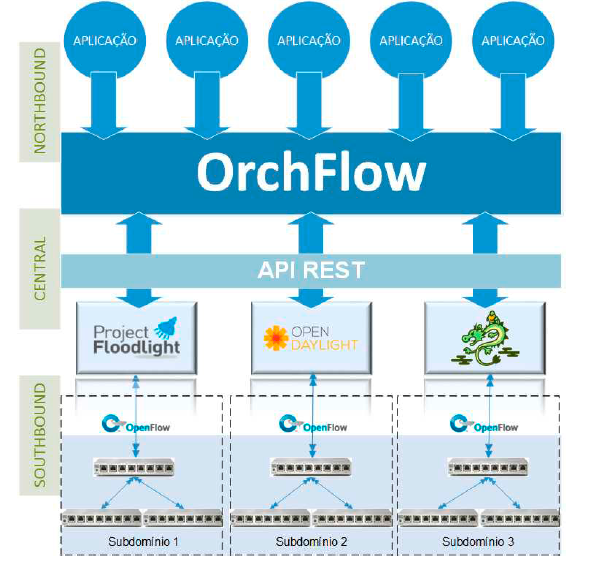
\includegraphics[scale= 0.8] {Imagens/orchflow.PNG} 
 
  \legend{Fonte: \citeonline{frate}}
  \label{orchflow}
\end{figure}

Com relação a sua implementação, a linguagem java foi escolhida para a implementação do OrchFlow. Além disso, para armazenamento dos dados, utiliza-se o banco de dados Neo4j \cite{neo}, um banco de dados orientado a grafos também baseado em Java, que oferece persistência, alto desempenho, escalabilidade e com boa documentação. 
\par A possibilidade da escalabilidade para gerenciar qualquer número de controladores implementados em qualquer linguagem, sob uma topologia hierárquica ou não e ainda com uma interface WEB torna o OrchFlow um orquestrador diferenciado, entretanto, seus testes ocorreram somente com os controladores Ryu e FLoodlight, sendo necessário mais testes para otimização de códigos com outros tipos de controladores, bem como com outros tipos de aplicações.













\include{Conteudo/Conclusao}

\bibliography{Bibliografia}

% ----------------------------------------------------------
% ELEMENTOS PÓS-TEXTUAIS
% ----------------------------------------------------------
\postextual

\renewcommand{\chapnumfont}{\chaptitlefont}
\renewcommand{\afterchapternum}{}
\begin{apendicesenv}

% Imprime uma página indicando o início dos apêndices
\partapendices

% ----------------------------------------------------------
\chapter{}
% ----------------------------------------------------------

\lipsum[50]

% ----------------------------------------------------------
\chapter{}
% ----------------------------------------------------------
\lipsum[55-57]

\end{apendicesenv}

\begin{anexosenv}


% Imprime uma página indicando o início dos anexos
\partanexos

% ---
\chapter{}
% ---
\lipsum[30]

% ---
\chapter{}
% ---

\lipsum[31]

% ---
\chapter{}
% ---

\lipsum[32]


\end{anexosenv}


\end{document}
